\documentclass[tikz,border=3pt]{standalone}
\usepackage[utf8]{inputenc}
\usepackage[T1]{fontenc}
\usepackage{lmodern}
\renewcommand{\familydefault}{\sfdefault}
\usepackage{sansmath}\sansmath
\usepackage{chemfig}
\usepackage{pgfplots}\pgfplotsset{compat=1.18,/pgf/number format/use comma,/pgf/number format/1000 sep={.}}
\usetikzlibrary{arrows.meta,calc,positioning,decorations.pathmorphing,patterns}
% paleta del sitio
\definecolor{nar}{HTML}{E8680C}\definecolor{narc}{HTML}{FFB35C}\definecolor{hielo}{HTML}{FFF3E8}
\definecolor{tinta}{HTML}{1D1D1F}\definecolor{gris}{HTML}{6E6E73}\definecolor{lila}{HTML}{7C5CF0}
\definecolor{azul}{HTML}{2F6FD6}\definecolor{menta}{HTML}{17A673}\definecolor{coral}{HTML}{E8342A}
\begin{document}
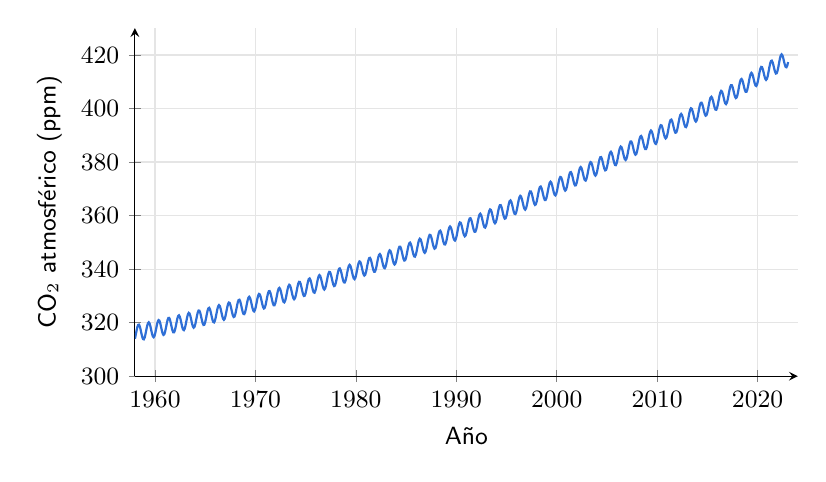
\begin{tikzpicture}[font=\small]
\begin{axis}[width=10cm,height=6cm,axis lines=left,xmin=1958,xmax=2024,ymin=300,ymax=430,xtick={1960,1970,...,2020},ytick={300,320,...,420},xticklabel style={/pgf/number format/1000 sep={}},xlabel={Año},ylabel={CO$_2$ atmosférico (ppm)},grid=major,grid style={gray!20}]
\addplot[azul,thick,domain=1958:2023,samples=800] {316 + 0.8*(x-1958) + 0.012*(x-1958)^2 + 3*sin(deg(2*pi*(x-1958.12)))};
\end{axis}
\end{tikzpicture}
\end{document}
